\chapter{METODOLOGI}

\section{Metode Penelitian}
\sloppy
Metode penelitian yang digunakan dalam penelitian ini adalah penelitian pengembangan dengan model pengembangan Richey dan Klein. Model ini terdiri dari tiga tahapan, yaitu \emph{Planning}, \emph{Production}, dan \emph{Evaluation} \cite{Sugiyono2019}. Setiap tahapan memiliki langkah-langkah spesifik yang harus diikuti untuk mencapai tujuan penelitian seperti pada diagram dibawah.

\begin{figure} [H] \centering
  % Nama dari file gambar yang diinputkan
  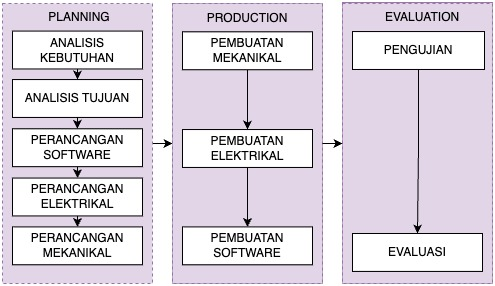
\includegraphics[scale=0.7]{gambar/method_diagram.jpg}
  % Keterangan gambar yang diinputkan
  \caption{Diagram alur penelitian}
  % Label referensi dari gambar yang diinputkan
  \label{fig:Diagram alur penelitian}
\end{figure}

\subsection{Perencanaan (\emph{Planning})}
Pada tahap ini, peneliti melakukan analisis dan perancangan prototipe. Analisis kebutuhan dilakukan untuk mengidentifikasi fitur dan spesifikasi yang diperlukan. Selain itu, analisis tujuan dilakukan untuk menentukan sasaran yang ingin dicapai dengan teknologi yang akan diterapkan. Berdasarkan hasil analisis kebutuhan dan tujuan, dilakukan perancangan prototipe yang mencakup perancangan perangkat lunak (\emph{software}), perancangan elektrikal, dan perancangan mekanikal.

\subsection{Produksi (\emph{Production})}
Tahap produksi mencakup pengembangan robot berdasarkan rencana yang telah dibuat. Pengembangan ini meliputi pembuatan komponen mekanikal, elektrikal, dan perangkat lunak (\emph{software}) sesuai dengan desain yang telah ditetapkan. Setiap komponen robot dikembangkan secara terintegrasi untuk memastikan kesesuaian dan kinerja sistem secara keseluruhan.

\subsection{Evaluasi (\emph{Evaluation})}
Pada tahap evaluasi, dilakukan pengujian secara bertahap untuk memastikan bahwa robot dapat beroperasi sesuai dengan tujuan yang telah ditetapkan. Pertama, dilakukan pengujian sub-sistem untuk memastikan setiap komponen sistem berfungsi dengan baik. Selanjutnya, pengujian terhadap fungsi-fungsi utama robot, seperti navigasi, deteksi \emph{overheat}, dan pengendalian jarak jauh, dilakukan untuk memastikan performa sistem secara keseluruhan. Terakhir, dilakukan pengujian di lingkungan nyata untuk menilai kinerja robot dalam kondisi operasional sesungguhnya. Jika ditemukan kekurangan atau masalah, perbaikan akan dilakukan untuk memastikan kinerja robot optimal dan sesuai dengan tujuan penelitian.


\section{Analisis Sistem}
Analisis dibagi menjadi analisis kebutuhan dan analisis tujuan seperti penjelasan berikut.

\subsection{Analisis Kebutuhan}
Analisis kebutuhan dilakukan melalui pengumpulan data dari studi literatur dan wawancara dengan pihak-pihak terkait. Berdasarkan hasil analisis, beberapa kebutuhan sistem yang harus dipenuhi adalah sebagai berikut:
\begin{enumerate}
  \item Sistem harus mampu mengidentifikasi komponen yang mengalami \emph{overheat} pada gardu listrik dengan menggunakan kamera termal, serta memberikan estimasi posisi dan jenis komponen yang terdeteksi.
  \item Sistem harus mampu melakukan patroli secara otonom di area gardu listrik, mengikuti jalur inspeksi yang telah ditentukan, dan menghindari rintangan fisik yang terdapat pada sekitar robot.
  \item Sistem harus dapat berkomunikasi secara \emph{online} dengan \emph{control station} untuk mengirimkan data posisi dan informasi deteksi robot secara real-time, serta menerima perintah kontrol seperti penetapan rute, jadwal patroli, serta perintah untuk melakukan \emph{wireless emergency stop} apabila terjadi keadaan darurat.
\end{enumerate}

\subsection{Analisis Tujuan}
Berdasarkan hasil analisis kebutuhan adapun tujuan yang ingin dicapai dalam pengembangan sistem ini adalah sebagai berikut:
\begin{enumerate}
  \item Mengembangkan sistem \emph{computer vision} untuk mendeteksi dan mengidentifikasi komponen yang mengalami \emph{overheat} menggunakan kamera termal. Sistem ini juga harus mampu memperkirakan posisi dan jenis komponen yang terdeteksi mengalami \emph{overheat}.
  \item Merancang dan mengimplementasikan sistem navigasi otonom pada robot, sehingga robot dapat melakukan patroli secara mandiri di area gardu listrik, menghindari rintangan fisik, dan mengikuti jalur inspeksi yang telah ditentukan. Sistem navigasi ini harus beroperasi dengan stabil dan akurat di lingkungan yang memiliki gangguan elektromagnetik serta interferensi dari peralatan listrik.
  \item Merancang dan membangun \emph{control station} yang dapat memantau lokasi robot dan hasil deteksi \emph{overheat} secara \emph{real-time}. Sistem ini harus dapat mengirim perintah kontrol \emph{emergency stop} secara \emph{wireless} ke robot. Selain itu, sistem harus dapat beroperasi secara online dan dapat diakses dari jarak jauh.
\end{enumerate}

\section{Desain Mekanikal}
Penelitian ini menggunakan robot \emph{quadruped legged} tipe \emph{DeepRobotics Jueying Lite 3 Pro} sebagai basis robot. Modifikasi dilakukan dengan menambahkan plat aluminium pada bagian atas robot sebagai tempat peletakan komponen. Plat aluminium ini dilapisi dengan cat isolator untuk mencegah terjadinya konduksi listrik, mengingat robot akan beroperasi di area gardu listrik.  Komponen tambahan yang dipasang meliputi kamera termal dan sensor LiDAR yang diletakkan di bagian depan robot, serta modul GPS, \emph{switch}, dan modem yang ditempatkan di dalam \emph{electrical box}. \emph{Electrical box} ini dirancang menggunakan teknologi \emph{3D printing} sebagai pelindung komponen elektronik dari benturan dan kerusakan akibat lingkungan eksternal.Desain mekanikal robot dirancang sedemikian rupa agar komponen tambahan dapat terpasang dengan aman tanpa mengganggu pergerakan robot. Seperti pada gambar \ref{fig:DesignMekanikalRobot},

\begin{figure}[H]
  \centering
  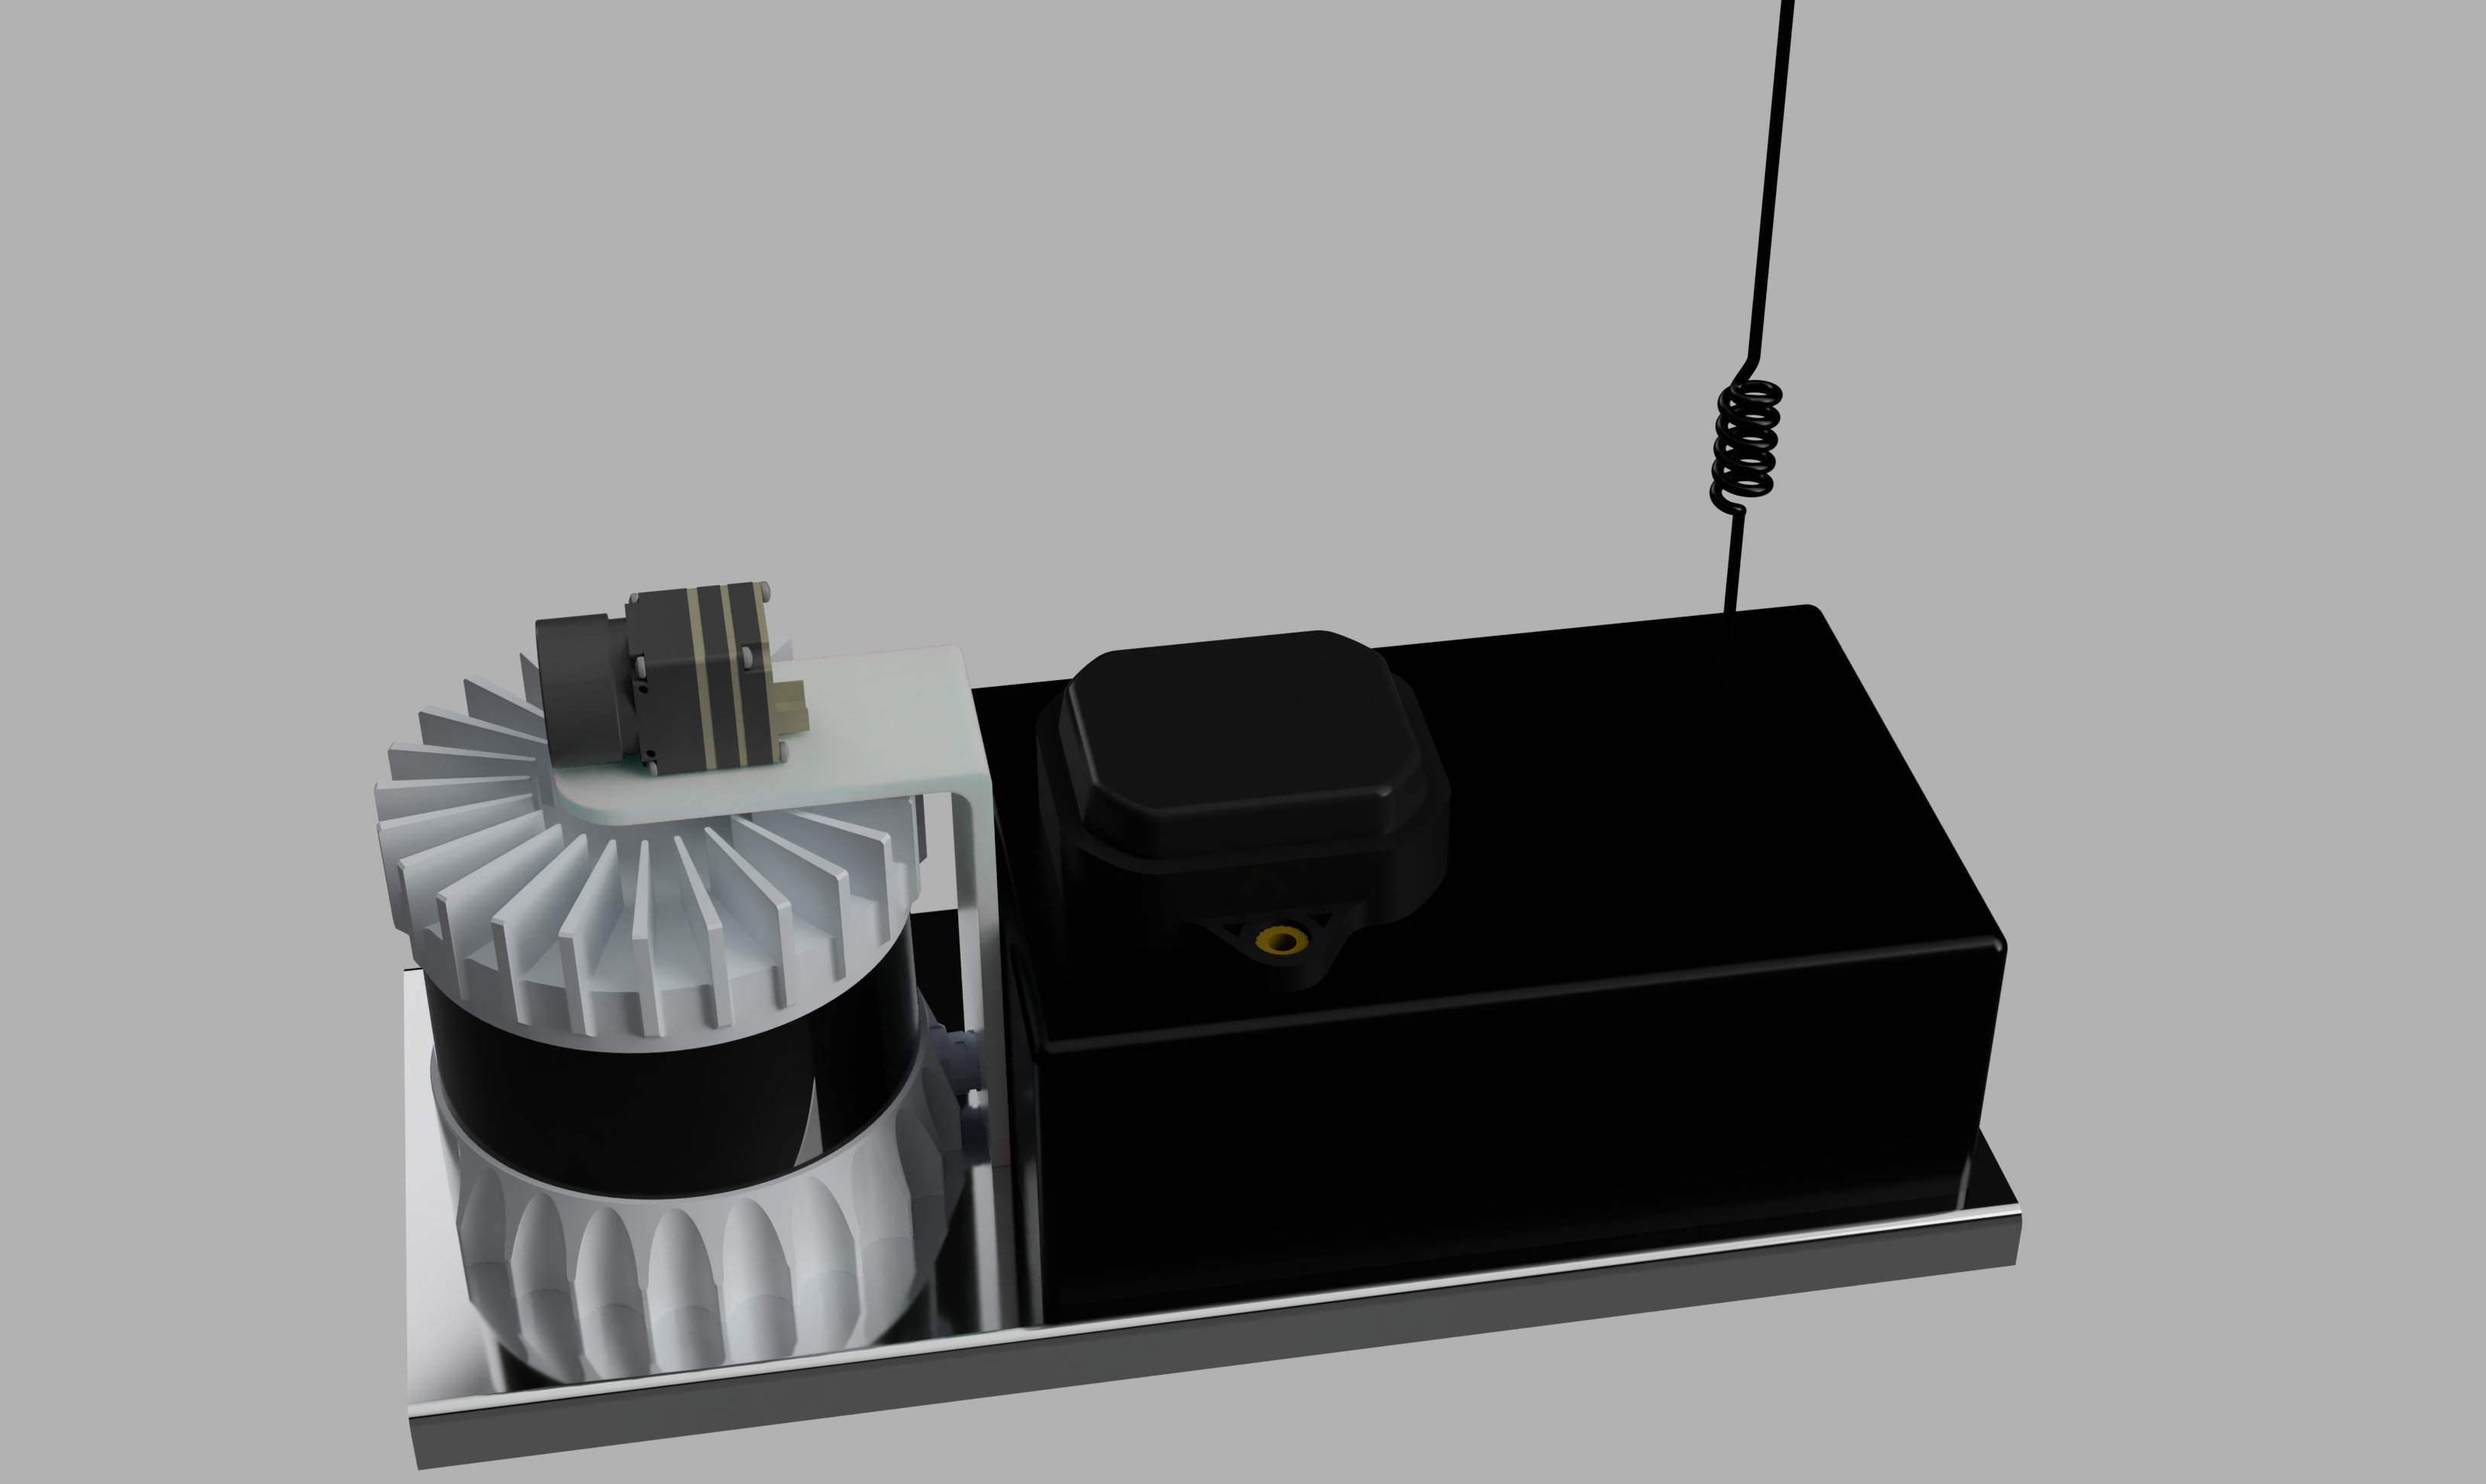
\includegraphics[scale=0.11]{gambar/mechanical_design.png}
  \caption{Desain komponen mekanikal robot}
  \label{fig:DesignMekanikalRobot}
\end{figure}

Penempatan sensor LiDAR di bagian atas robot memungkinkan sensor untuk memperoleh pandangan yang lebih luas, sedangkan kamera termal ditempatkan di posisi strategis untuk mendeteksi perubahan suhu pada komponen gardu listrik. \emph{Electrical box} dipasang di bagian belakang robot untuk mengoptimalkan distribusi berat dan memastikan kestabilan robot.

\section{Desain Elektrikal}

Desain elektrikal robot mencakup perancangan sistem distribusi daya dan komunikasi yang bertujuan untuk mengintegrasikan komponen-komponen tambahan ke dalam sistem robot yang sudah ada. Komponen-komponen tambahan tersebut dirancang untuk mendukung kemampuan operasi otonom robot. Desain elektrikal lengkap dari robot ini dapat dilihat pada Gambar \ref{fig:Desain electrical robot}.

\begin{figure}[H] \centering
  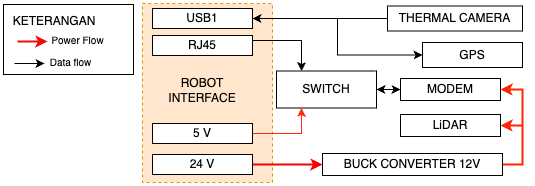
\includegraphics[scale=0.72]{gambar/electrical.png} \caption{Desain \emph{block diagram} sistem distribusi daya dan komunikasi elektrikal robot} 
   \label{fig:Desain electrical robot} 
\end{figure}

Dalam hal distribusi daya, tegangan 24V yang disuplai oleh robot diturunkan menjadi 12V menggunakan modul \emph{buck converter} untuk memenuhi kebutuhan daya LiDAR dan modem. Komponen lain yang memerlukan tegangan 5V memperoleh catu daya dari sumber 5V yang tersedia pada robot. Selain itu, terdapat modul GPS dan \emph{thermal camera} yang terhubung melalui port USB. Sementara itu, LiDAR dan modem terhubung melalui switch dan kemudian masuk ke dalam sistem robot melalui LAN. Sistem komunikasi menggunakan protokol \emph{wireless} melalui modem yang terhubung ke jaringan \emph{BTS provider} untuk mengirimkan data posisi dan informasi deteksi \emph{overheat} ke \emph{control station}.

\section{Arsitektur Perangkat Lunak Robot}
Arsitektur perangkat lunak robot menggunakan \emph{Robot Operating System (ROS) 1 Noetic}, ROS berfungsi sebagai \emph{middleware} untuk mendukung pengembangan program secara modular. ROS memfasilitasi pengembangan dengan menggunakan \emph{package} dan \emph{node} yang saling berinteraksi, sehingga memungkinkan pengembangan yang efisien dan terstruktur. Pemilihan ROS 1 Noetic didasarkan pada kompatibilitasnya dengan robot \emph{DeepRobotics Jueying Lite 3}. Integrasi ini memungkinkan sistem navigasi yang dirancang untuk memerintahkan robot bergerak pada sumbu translasi \(x\), \(y\), dan sumbu rotasi \(z\) (\emph{angular z}) dengan nilai kecepatan tertentu tanpa perlu mengembangkan ulang program \emph{kinematic} atau kontrol pergerakan robot yang sudah ditangani oleh program bawaan \emph{DeepRobotics Jueying Lite 3}. Arsitektur perangkat lunak pada robot dapat dibagi dibagi menjadi tiga \emph{package}, yaitu \emph{hardware interface}, dan \emph{control}, \emph{perception}. Desain arsitektur perangkat lunak robot dapat dilihat pada Gambar \ref{fig:Desain perangkat lunak robot}.

\begin{figure}[H] \centering
  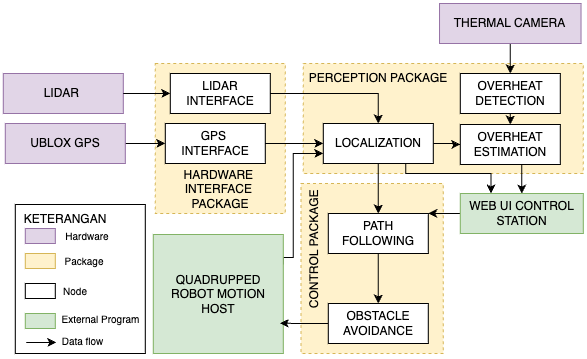
\includegraphics[scale=0.7]{gambar/software.png}
  \caption{Desain arsitektur perangkat lunak robot} 
  \label{fig:Desain perangkat lunak robot}
\end{figure}

Berdasarkan gambar diatas dapat dilihat \emph{HARDWARE INTERFACE} akan memberikan data GPS, LiDAR, dan IMU yang diperoleh dari sensor GPS dan LiDAR ke \emph{PERCEPTION}. \emph{PERCEPTION} akan menggabungkan data dari \emph{HARDWARE INTERFACE} dengan \emph{odometry} yang diperoleh dari \emph{MOTION HOST} untuk mendeteksi posisi dan orientasi robot dalam peta. Selain itu, \emph{PERCEPTION}. \emph{PERCEPTION}  juga akan memproses data dari kamera termal untuk mendeteksi adanya \emph{overheat} pada komponen gardu listrik serta memperkirakan posisi komponen yang mengalami \emph{overheat}. Hasil deteksi dari \emph{PERCEPTION} akan dikirim ke \emph{CONTROL STATION} melalui \emph{websocket}, dan \emph{PERCEPTION} juga akan melakukan \emph{broadcast} posisi robot (\emph{TF}) dan marker LiDAR ke map.  Disisi lain \emph{CONTROL STATION} akan menerima data posisi dan lokasi dari \emph{PERCEPTION} serta rute yang dikirim oleh \emph{CONTROL STATION}. Ketika perintah \emph{start} diterima dari \emph{CONTROL STATION}, robot akan merencanakan trajektori untuk melakukan patroli sambil menghindari \emph{obstacle} yag ada pada rute. Data trajektori kemudian akan dikirim ke \emph{MOTION HOST} untuk menggerakkan robot. 

\subsection{\emph{Hardware Interface Package}}
\emph{Hardware interface} mengelola interaksi dengan sensor. \emph{Package} ini terdiri dari dua \emph{node} dengan tugas masing-masing. Node pertama, \emph{GPS Interface}, membaca data dari sensor GPS dan menjalankan \emph{Real Time Kinematic} (RTK) untuk menghubungkan sensor GPS robot dengan stasiun basis, memberikan koreksi sinyal satelit dan memungkinkan pengukuran posisi yang lebih presisi. Node kedua, \emph{LiDAR Interface}, membaca data sensor LiDAR dan mengirimkan \emph{point cloud} ke \emph{perception}, yang merepresentasikan objek di sekitar robot.

\subsection{Perception}
\emph{Perception} adalah \emph{package} yang berfungsi untuk memproses data sensor guna memungkinkan robot memahami lingkungan sekitarnya. \emph{Package} ini terdiri dari beberapa \emph{node} utama, yang masing-masing memiliki fungsi tertentu diantaranya adalah sebagai berikut.

\subsubsection{\emph{Localization Node}}
Dalam penelitian ini, robot menggunakan \emph{predefined topological map}, yang diambil dari Google Maps atau aplikasi lainnya. Posisi awal robot atau \emph{initial state} ditentukan pada titik tetap (\emph{fixed position}) dalam peta topologi yang telah ditentukan sebelumnya. Dalam menentukan orientasi, sistem ini menggunakan data \emph{IMU}, \emph{GPS}, dan \emph{LiDAR} yang didapat dari \emph{HARDWARE INTERFACE} untuk menghitung orientasi robot dalam peta topologi. Untuk menentukan posisi robot, digunakan dua metode utama, yaitu \emph{GPS} dan \emph{Direct LiDAR Inertial Odometry} (DLIO). Metode \emph{GPS} digunakan untuk menentukan posisi robot dalam koordinat geografis. Namun, di area yang dipenuhi dengan interferensi elektromagnetik, seperti gardu listrik, sinyal \emph{GPS} dapat terpengaruh, sehingga menurunkan kualitas akurasi di beberapa kondisi. Untuk mengatasi hal ini, jika sinyal \emph{GPS} terdeteksi berada di bawah ambang batas akurasi yang dibutuhkan, sistem secara otomatis beralih menggunakan metode \emph{Direct LiDAR Inertial Odometry} (DLIO). \emph{DLIO} menggabungkan informasi dari sensor \emph{LiDAR} dan \emph{IMU} (\emph{Inertial Measurement Unit}) yang digabungkan dengan odometri dengan menggunakan \emph{Extended Kalman Filter} (EKF) untuk menghitung posisi dan orientasi robot.

\subsubsection{\emph{Overheat Detection Node}}
\emph{Node} ini berfungsi untuk mendeteksi komponen yang mengalami suhu tinggi (\emph{overheat}) menggunakan kamera termal yang terpasang pada robot. Citra termal yang diperoleh diklasifikasikan menggunakan \emph{YOLOv8} untuk mendeteksi komponen gardu listrik. Setelah komponen terdeteksi, analisis suhu dilakukan pada bounding box menggunakan teknik kontur dengan threshold warna pada ruang warna HSV (\emph{Hue}, \emph{Saturation}, \emph{Value}). Thresholding dilakukan pada saluran \emph{HSV} untuk mengidentifikasi suhu tinggi, dan kontur diterapkan untuk memetakan area yang menunjukkan suhu berlebih. Jika suhu komponen melebihi ambang batas, komponen tersebut diklasifikasikan sebagai \emph{overheat}.

\subsection{\emph{Overheat pose estimation Node}}
\emph{Node} ini berfungsi untuk mendeteksi posisi komponen yang mengalami \emph{overheat}. Setelah komponen yang mengalami \emph{overheat} terdeteksi, \emph{node} ini akan memperkirakan posisi komponen tersebut dalam peta topologi. Posisi komponen diestimasi berdasarkan posisi robot yang diperoleh dari \emph{Localization Node} dan data LiDAR yang diperoleh dari \emph{HARDWARE INTERFACE}. Data LiDAR digunakan untuk memetakan area sekitar robot dan mengidentifikasi posisi relatif komponen yang mengalami \emph{overheat} terhadap posisi robot. Hasil estimasi posisi kemudian dikirim ke \emph{CONTROL STATION} untuk ditampilkan pada \emph{graphical user interface (GUI)}.

\subsection{\emph{Control}}
\emph{Control} adalah \emph{package} yang berfungsi untuk mengelola pergerakan robot. \emph{Package} ini terdiri dari beberapa \emph{node} utama, diantaranya adalah sebagai berikut.

\subsubsection{\emph{Patrol Control Node}}

\emph{Node} ini berfungsi sebagai otak
 dari robot yang bertanggung jawab untuk mengatur pergerakan robot berdasarkan perintah yang diterima dari \emph{CONTROL STATION}. Perintah yang diterima meliputi perintah untuk memulai patroli, menghentikan patroli, dan mengubah rute patroli. \emph{Patrol Control Node} akan merencanakan trajektori robot berdasarkan rute yang diterima berupa \emph{waypoint} dan mengirimkan perintah ke \emph{MOTION HOST} untuk menggerakkan robot. Dalam mengikuti \emph{waypoint}, robot akan menggunakan algoritma \emph{path following} yang dibuat oleh Akbar 2022. Algoritma ini menggunakanposisi dan orientasi dari \emph{Localization Node} sebagai referensi kontrol. Pada kontrol ini terdapat \emph{WaypointControl}, yang berperan untuk mengarahkan robot menuju titik yang ditentukan. Adapun rumus error yang digunakan dapat dilihat pada Persamaan \ref{eq:error}. Representasi error yang dimaksud dijelaskan melalui Gambar \ref{fig:error_waypointcontrol} \cite{zidan2022}.

\begin{figure}[H] \centering
  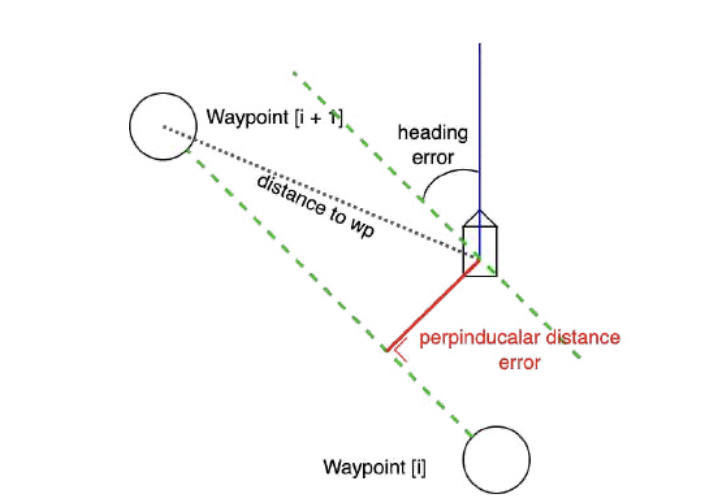
\includegraphics[scale=0.8]{gambar/waypoint_control.png}
  \caption{Representasi error pada \emph{WaypointControl}}
  \label{fig:error_waypointcontrol}
\end{figure}

\begin{equation}
  \label{eq:error}
  \mathrm{error} = \mathrm{heading}_{\mathrm{error}} + \mathrm{perpendicular\ distance}_{\mathrm{error}}.
\end{equation}

Adapun kondisi dimana waypoint telah tercapai adalah apabila kondisi berikut ini terpenuhi:

\begin{equation}
  \label{eq:condition_distance}
  \mathrm{distance\ to\ wp} < \mathrm{threshold\ distance}.
\end{equation}

\begin{equation}
  \label{eq:condition_angle}
  \mathrm{angle\ to\ wp} > \mathrm{threshold\ angle}.
\end{equation}

Error yang didapat kemudian di proses dengan menggunakan \emph{PID controller} untuk mendapatkan output pergerakan robot yang akan dikirim ke \emph{MOTION HOST}.

\subsubsection{\emph{Obstacle Avoidance Node}}
\emph{Obstacle Avoidance Node} bertugas untuk mendeteksi obyek pada rute dan menghindari tabrakan saat mengikuti \emph{waypoint}. Robot menggunakan data LiDAR dari \emph{HARDWARE INTERFACE}, yang diproses dengan algoritma \emph{Braitenberg} untuk mendeteksi obyek. Algoritma ini menghasilkan nilai \emph{gain} yang mengatur kecepatan robot dalam menghindari obyek. Jika obyek terdeteksi, robot akan mengurangi kecepatan atau mengubah arah. Setelah obyek tidak terdeteksi, robot akan kembali ke rute dan melanjutkan pergerakan menuju \emph{waypoint} berikutnya.

\section{Desain Antarmuka Pengguna (\emph{User Interface}) Sistem Kontrol}

Sistem ini menggunakan antarmuka berbasis web GUI yang dibangun dengan \emph{Next.js 14} dan \emph{roslibjs} untuk integrasi dengan ROS. Sistem akan di-\emph{deploy} pada internet menggunakan \emph{Node.js}. \emph{PostgreSQL} digunakan sebagai database, sementara \emph{Prisma} berfungsi sebagai \emph{ORM} untuk mengelola data. Sistem GUI dapat dibagi menjadi tiga bagian utama yang memiliki fungsi sebagai berikut:

\subsection{\emph{Authentication Page}}

\emph{Authentication Page} adalah halaman yang ditampilkan kepada pengguna yang ingin mengakses sistem. Sistem ini menggunakan \emph{next/auth} untuk mengelola autentikasi pengguna. Pengguna dapat mendaftarkan akun melalui formulir pendaftaran. Setelah proses pendaftaran, \emph{next/auth} akan mengelola autentikasi dan menyimpan data pengguna di \emph{PostgreSQL}.

\subsection{\emph{Robot Information}}

\emph{Robot Information} adalah halaman yang menampilkan informasi terkait robot, seperti nama, versi, dan spesifikasi dari robot yang terdaftar dalam sistem. Halaman ini juga menampilkan status real-time robot, termasuk posisi, kecepatan, dan arah gerak. Pengguna dapat mendaftarkan robot baru melalui halaman ini, sehingga robot dapat terdaftar dan digunakan dalam sistem. Setiap robot yang didaftarkan akan memiliki ID unik yang digunakan untuk mengidentifikasi robot tersebut di seluruh sistem.

\subsection{\emph{Patrol Controller}}

\emph{Patrol Controller} adalah halaman utama yang digunakan untuk mengontrol robot dan memantau operasi patroli. Sistem ini mendukung operasi multi-robot, sehingga setiap robot yang terdaftar akan memiliki \emph{Patrol Controller} masing-masing. Halaman ini menampilkan peta interaktif yang menunjukkan posisi robot, rute patroli, dan status \emph{real-time} robot. Selain itu, citra termal robot juga ditampilkan untuk mendeteksi komponen yang mengalami \emph{overheat}. 

Pengguna dapat memilih robot yang ingin dikontrol menggunakan ID robot yang telah didaftarkan di \emph{Robot Information}. Setiap robot memiliki kontrol manual dan otomatis melalui tombol yang tersedia di halaman ini. Di \emph{Patrol Controller}, pengguna juga dapat membuat atau mengubah rute patroli dan menetapkan jadwal patroli untuk setiap robot secara terpisah. Dengan sistem multi-robot ini, pengguna dapat memantau dan mengelola beberapa robot secara bersamaan, masing-masing dengan kontrol dan informasi yang terpisah berdasarkan ID robot yang dipilih.

\section{\emph{Computer Vision}}

Dalam mendeteksi komponen yang mengalami \emph{overheat}, peneliti menggunakan model \emph{YOLOv8}. Pemilihan model ini didasarkan pada kemampuannya dalam deteksi objek yang akurat dan kecepatan proses yang optimal. Proses deteksi komponen \emph{overheat} dilakukan melalui beberapa tahapan sebagai berikut:

\subsection{Pembuatan Dataset}
Dataset citra termal dari komponen gardu listrik dikumpulkan dan diproses untuk melatih model deteksi. Pengumpulan data dilakukan melalui platform \emph{Roboflow}, di mana setiap citra diberi label secara akurat untuk mengidentifikasi jenis komponen yang terdeteksi.

\subsection{Pelatihan Model \emph{YOLOv8}}
Model \emph{YOLOv8} dilatih menggunakan dataset yang telah disiapkan. Proses pelatihan mencakup penyesuaian hiperparameter dan penggunaan augmentasi data untuk meningkatkan akurasi model. Evaluasi kinerja model dilakukan dengan menggunakan metrik \emph{mean Average Precision} (mAP) dan \emph{Intersection over Union} (IoU) untuk menilai kemampuan deteksi. Setelah pelatihan, model diuji menggunakan dataset validasi untuk memastikan kinerja yang optimal.

\subsection{Konversi ke \emph{TensorRT}}
Untuk meningkatkan kecepatan deteksi dan mengurangi beban komputasi, model \emph{YOLOv8} dikonversi ke format \emph{TensorRT} (TRT). Model yang awalnya dalam format \emph{PyTorch} diekspor ke format \emph{Open Neural Network Exchange} (ONNX) menggunakan perintah dari \emph{library Ultralytics}. Setelah model diekspor ke format ONNX, konversi ke format TRT dilakukan dengan perintah \texttt{trtexec} dari NVIDIA untuk mempercepat proses inferensi.

\subsection{Deteksi Suhu Komponen}
Setelah komponen berhasil terdeteksi oleh \emph{YOLOv8}, tahap selanjutnya adalah menganalisis suhu pada komponen dengan menggunakan segmentasi warna dalam ruang warna \emph{HSV} (\emph{Hue, Saturation, Value}) pada \emph{bounding box} yang terdeteksi. Metode ini digunakan untuk mengidentifikasi area dalam citra termal yang memiliki suhu tinggi, biasanya ditunjukkan dengan warna seperti merah, kuning, atau oranye, sesuai dengan dataset kamera termal yang digunakan.

Deteksi komponen terlebih dahulu sangat penting karena setiap komponen memiliki ambang batas suhu \emph{overheat} yang berbeda. Tanpa mengetahui jenis komponen yang terdeteksi, sulit untuk menentukan apakah suhu tersebut melebihi batas aman atau tidak. Oleh karena itu, identifikasi komponen terlebih dahulu memastikan bahwa segmentasi suhu yang dilakukan pada \emph{bounding box} yang terdeteksi relevan dan akurat. Berdasarkan data ambang batas suhu masing-masing komponen.

